\documentclass{VUMIFPSbakalaurinis}
\usepackage{algorithmicx}
\usepackage{algorithm}
\usepackage{algpseudocode}
\usepackage{amsfonts}
\usepackage{amsmath}
\usepackage{bm}
\usepackage{caption}
\usepackage{color}
\usepackage{float}
\usepackage{graphicx}
\usepackage{listings}
\usepackage{subfig}
\usepackage{wrapfig}

\usepackage{enumitem}
\setitemize{noitemsep,topsep=0pt,parsep=0pt,partopsep=0pt}
\setenumerate{noitemsep,topsep=0pt,parsep=0pt,partopsep=0pt}

\hbadness=100000
% Titulinio aprašas
\university{Vilniaus universitetas}
\faculty{Matematikos ir informatikos fakultetas}
\department{Programų sistemų studijų programa}
\papertype{Mokslo tiriamasis darbas III}
\title{Srautinio apdorojimo sistemų balansavimas taikant mašininį mokymąsi}
\titleineng{Balancing stream processing systems using machine learning}
\author{Vytautas Žilinas}
\supervisor{Andrius Adamonis}
\reviewer{Prof. dr. Aistis Raudys}
\date{Vilnius – \the\year}

% Nustatymai
% \setmainfont{Palemonas}   % Pakeisti teksto šriftą į Palemonas (turi būti įdiegtas sistemoje)
\bibliography{bibliografija}

\begin{document} 
\maketitle

\cleardoublepage\pagenumbering{arabic}
\setcounter{page}{2}

\tableofcontents

\sectionnonum{Įvadas}

Realaus laiko duomenų apdorojimas (angl. real–time data processing) yra jau senai nagrinėjamas kaip vienas iš būdų apdoroti didelių kiekių duomenis (angl. Big data). Vienas iš realaus laiko apdorojimo sprendimų yra srautinis duomenų apdorojimas. Srautinis duomenų apdorojimas (angl. stream processing) – lygiagrečių programų kūrimo modelis, pasireiškiantis sintaksiškai sujungiant nuoseklius skaičiavimo komponentus srautais, kad kiekvienas komponentas galėtų skaičiuoti savarankiškai \cite{shortstreamproc}. 

Yra keli pagrindiniai srautinio apdorojimo varikliai: „Apache Storm“, „Apache Spark“, „Heron“ ir kiti. „Apache Storm“ ir „Heron“ apdoroja duomenis duomenų srautais, o „Apache Spark“ mikro–paketais \cite{karau2015learning}. „Heron“ srautinio apdorojimo variklis, buvo išleistas „Twitter“ įmonės 2016 metais kaip patobulinta alternatyva „Apache Storm“ srautinio apdorojimo varikliui \cite{openSourcing}. Šiame darbe bus naudojamas „Heron“, kadangi tai yra naujesnis ir greitesnis srautinio apdorojimo variklis nei „Apache Storm“ \cite{twitterHeron}. 

Srautinio apdorojimo sistemų balansavimas (angl. auto–tuning) – tai sistemos konfigūracijos valdymas siekiant užtikrinti geriausią resursų išnaudojimą – duomenų apdorojimas neprarandant greičio, bet ir naudojant tik reikiamą kiekį resursų. Kadangi srautinio apdorojimo sistemų komponentai yra kuriami kaip lygiagretus skaičiavimo elementai, todėl jie gali būti plečiami horizontaliai ir vertikaliai \cite{shortstreamproc} keičiant sistemų konfigūraciją. Tačiau lygiagrečių elementų kiekio keitimas nėra vienintelis būdas optimizuoti resursų išnaudojimą. Kiekvienas variklis turi savo rinkinį konfigūruojamų elementų. Darbe naudojamas „Heron“ variklis leidžia optimizuoti sistemas naudojant 56 konfigūruojamus parametrus \cite{configDocument}.

Yra skirtingi būdai kaip gali būti parenkama tinkama konfigūracija. Kadangi dar nėra naudojimui paruoštų sprendimų, kurie galėtų balansuoti srautinio apdorojimo sistemas savarankiškai, dažniausiai už tai yra atsakingi inžinieriai, kurie dirba su šiomis sistemomis. Kadangi srautinio apdorojimo sistemų apkrovos gali būti skirtingų pobūdžių (duomenų kiekis, skaičiavimų sudėtingumas, nereguliari apkrova), o inžinieriai konfigūruodami išbando tik kelis derinius ir pasirenka labiausiai tinkanti \cite{selfRegulatingStreaming}, lieka labai daug skirtingų neišbandytų konfigūracijos variacijų. Optimalios konfigūracijos suradimas yra NP sudėtingumo problema \cite{automateTuning}, kadangi žmonėms yra sunku suvokti didelį kiekį konfigūracijos variacijų. 
Vienas iš būdų automatiškai valdyti konfigūraciją buvo pasiūlytas 2017 metų straipsnyje „Dhalion: self–regulating stream processing in heron“, kuriame autoriai aprašo savo sukurtą sprendimą „Dhalion“, kuris konfigūruoja „Heron“ srautinio apdorojimo sistemas pagal esamą apkrova ir turimus resursus, t.y. jei apdorojimo elementų išnaudojimas išauga >100\%, „Dhalion“ padidina lygiagrečiai dirbančių apdorojimo elementų kiekį \cite{dhalion}. Tačiau šis sprendimas leidžia reguliuoti tik elementų lygiagretumą ir tai daro tik reaktyviai.
Vienas iš naujausių būdų balansuoti srautinio apdorojimo sistemas – mašininis mokymasis. Vienas iš tokių bandymų aprašytas 2018 metų straipsnyje „Auto–tuning Distributed Stream Processing Systems using Reinforcement Learning“, kuriame atliktas tyrimas – „Apache Spark“ sistemos balansavimui naudojamas skatinamojo mokymo REINFORCE algoritmas, kuris, pagal dabartinę konfigūraciją ir renkamas metrikas, keitė srautinio apdorojimo sistemos konfigūracijos parametrus. Šiame tyrime nustatyta, jog sprendimas, naudojantis mašininį mokymąsi, suranda optimalesnę konfigūraciją per trumpesnį laiką nei žmones ir taip pat surastą konfigūraciją naudojančios srautinio apdorojimo sistemos vėlinimas (angl. latency) yra 60–70\% mažesnis nei tyrimo metu ekspertų derinamos konfigūracijos \cite{vaquero2018autotuning}. Šiame darbe naudojamas „Heron“ variklis leidžia prie savęs prijungti sukurtą išorinę metrikų surinkimo programą, kuri gali rinkti tokias sistemų metrikas kaip: naudojama RAM atmintis, CPU apkrova, komponentų paralelizmas ir kitas, kurios gali būti naudojamos balansavimui. 

Skatinamasis mokymasis yra vienas iš mašininio mokymosi tipų. Šis mokymasis skiriasi nuo kitų, nes nereikia turėti duomenų apmokymui, o programos mokosi darydamos bandymus ir klysdamos. Pagrindinis uždavinys naudojant skatinamąjį mokymąsi – surasti balansą tarp naujų sprendimų tyrinėjimo (angl. exploration) ir turimos informacijos išnaudojimo (angl. exploitation) \cite{reinforcment}. Vienas iš pagrindinių privalumų naudojant skatinamąjį mokymąsi balansavimui – nereikia turėti išankstinių duomenų apmokymui kas leidžia jį paprasčiau pritaikyti skirtingoms srautinio apdorojimo sistemų apkrovoms. Tačiau tokio tipo mašininis mokymasis turi ir problemų: sudėtinga aprašyti tinkamos konfigūracijos apdovanojimo (angl. reward) funkciją ir balansą tarp tyrinėjimo ir išnaudojimo tam, kad nebūtų patiriami nuostoliai \cite{selfRegulatingStreaming}.

Yra sukurta daug skatinamojo mokymosi algoritmų (Monte Carl, Q–learning, Deep Q Network ir kiti), šiame darbe jie bus apžvelgti ir vienas iš jų bus pasirinktas ir pritaikytas išsikeltam uždaviniui. 

Numatomas magistro darbo tikslas: Ištirti mašininio mokymosi tinkamumą srautinio apdorojimo sistemų balansavimui. 

Numatomi magistro darbo uždaviniai:
\begin{enumerate}
    \item Sudaryti srautinio apdorojimo sistemų balansavimo modelį ir nustatyti valdymo metrikas irjų siekiamas reikšmes, kurios bus naudojamos eksperimentinėje sistemoje.
    \item Parinkti skatinamojo mokymosi algoritmą eksperimentui, atsirenkant iš algoritmų, aprašomų literatūroje.
    \item Sukurti eksperimentinį sprendimą su pasirinktu algoritmu ir atlikti eksperimentus.
    \item Palyginti eksperimento rezultatus su alternatyvomis - „Heron“ su standartine konfigūracija, „Heron“ su „Dhalion“ priedu bei „Heron“ balansavimas pritaikius REINFORCE algoritmą. 
\end{enumerate}


\subsection*{Šio darbo tikslas ir uždaviniai}
Tikslas: apibrėžti darbo metodą ir sukurti bei pagrįsti algoritmą, kuris bus naudojamas eksperimentui.

Uždaviniai:
\begin{enumerate}
    \item Apibrėžti algoritmą srautinio apdorojimo sistemų balansavimui naudojanti Deep Q Network ir Actor-Critic skatinamojo mokymosi algoritmus.
    \item Apibrėžti eksperimento eigą ir altenatyvius sprendimus, kurių rezultatai bus naudojami algortimo įvertinimui. 
\end{enumerate}

\section{Srautinio apdorojimo sistemų balansavimo algoritmas}
Šiame skyriuje aptariamas algoritmas, kuris bus naudojamas srautinių sistemų balansavimui. 
\begin{figure}[H]
    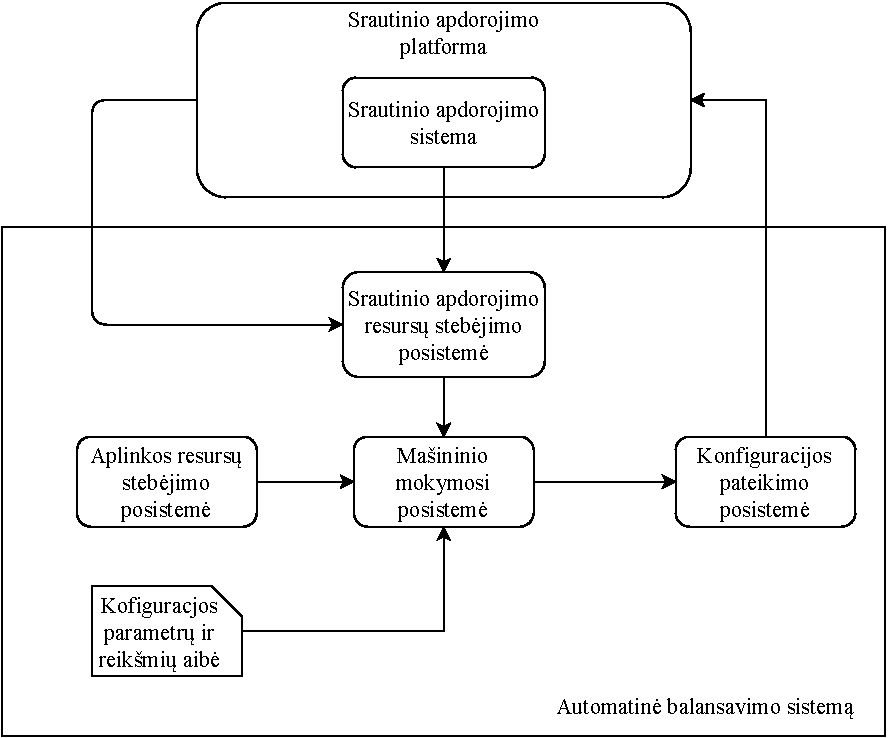
\includegraphics[width=15cm]{img/BalansavimoDiagrama.pdf}
    \caption{Pagrindiniai algoritmo elementai ir jų tarpusavio ryšiai}
    \label{balansavimo_sistema}
\end{figure} 

\subsection{Tikslas}
Algoritmo tikslas savarankiškai reguliuoti srautinio apdorojimo sistemos konfiguracijos parametrus siekiant palaikyti sistemą stablią ir optimaliai naudojančia resursus. \ref{balansavimo_sistema} pav. pavazduota sistema yra integruojama į srautinio apdorojimo sistemos platformą iš kurios ji gauna reikiamą informacija apie srautinio apdorojimo sistemos metrikas ir resursus, bei turėti informaciją apie esamus aplinkos naudojamus ir turimus resursus. Balansavimo algoritmas eksperimente bus implementuojamas kaip posistemė, kuri gauna metrikas iš srautinio apdorojimo sistemos platformos ir operacinės sistemos, o atnaujintą konfiguraciją pateikia į srautinio apdorojimo platformą per komandų įvedimo eilutę.

\subsection{Įeiga}
Kad mašinio mokymosi posistemė galėtų daryti sprendimus, jai paduodami šie duomenys:
\begin{itemize}
    \item Srautinio apdorojimo sistemos naudojami resursai ir metrikos – procesoriaus apkrova, operatyviosios atminties apkrova, priešslėgis (angl. backpressure), srautinio apdorojimo sistemos įeigos komponento atsilikimas nuo duomenų srauto.
    \item Aplinkos naudojami resursai – procesoriaus apkrova, operatyviosios atminties apkrova.
    \item Srautinio apdorojimo sistemos pradinė konfiguracija - komponentų lygiagretumo parametrai, konteinerių parametrai, konfiguracijos elementai ir jų reikšmės.
    \item Konfiguruojami parametrai ir jų reikšmių ribos.
    \item Mašinio mokymosi algoritmo konfiguracija - sprendimų priemimo periodiškumas.
    \item Buvusio ciklo pradiniai duomenys ir priimti sprendimai.
\end{itemize}

\subsection{Eiga}

Sistema naudojanti mašininį mokymąsi veikia pastoviai vienodo periodo ciklais (\ref{veikimas} pav.). 
\begin{figure}[H]
    \centering
    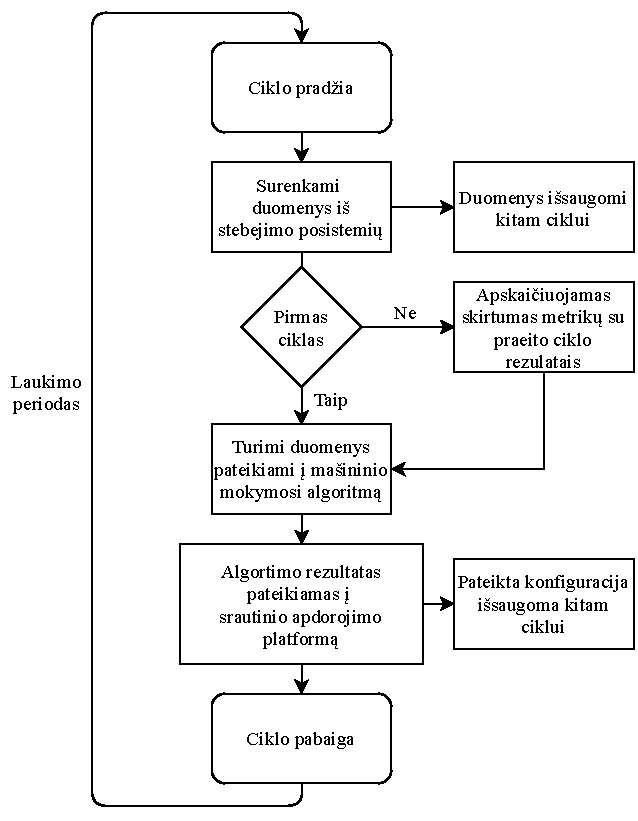
\includegraphics[width=10cm]{img/AlgoritmoVeikimas.pdf}
    \caption{Algortimo veikimas}
    \label{veikimas}
\end{figure} 
Tarpas tarp ciklų apibrežiamas leidžiant balansavimo sistemai ir yra skirtas srautinio apdorojimo sistemai atsinaujinti su naujais konfiguracijos parametrais bei kad surinkti duomenys būtų pakankamai svarūs pateikti į mašininį mokymosi algoritmą.

\subsection{Algoritmo rezultatas}
Mašinio mokymosi posistemė, atlikusi skaičiavimus, gražiną naują konfiguracijos parametrų rinkinį, kuris yra veliau pateikiamas į srautinio apdorojimo sistemų platformą. Po srautinės apdorojimo sistemos pradedamas naujas ciklas sistemos stebėjimo ir naujų konfiguracijos parametrų kurimo, kuris taip pat atsižvelgia į metrikų skirtumo ir konfiguracijos pakeitimo rezultatus iš  ankstesnių ciklų.

\subsection{Algoritmui tikrinti naudojami skatinamojo mokymosi algoritmai}
Šiame skyriuje bus aprašomi skatinamojo mokymosi algoritmai, kurie bus naudojami eksperimentui. Šie algoritmai pasirinkti pagal MTD II literatūros analizę, tačiau pats balansavimo algoritmas yra nepriklausomas nuo naudojamo skatinamojo mokysimosi algortimų ir gali būti įgyvendintas naudojant kitus algoritmus.
\subsection{Deep Q Network}

\subsection{Actor-Critic}

\section{Alternatyvus sprendimai}
Siekiant užtikrinti sprendimo validumą ir efektyvumą bus atliekamas eksperimentas ir rezultatai bus lyginamį su alternatyviais sprendimais.

\subsection{Rezultatų surinkimas}

Pagal literatūros analizę atlikta MTDII matoma, kad dauguma autorių renkasi vertinti tik pagal vieną metriką ir dažniau matavimui naudojamas vėlinimas (angl. latency). Taip pat \cite{vaquero2018autotuning}, naudojantis skatinamąjį mokymą, matavimui naudoja vėlinimą ir \cite{Chintapalli2016Benchmarking} straipsnis, kuris siūlo srautinio apdorojimo sistemų vertinimo sprendimą, naudoja vėlinimą. Todėl eksperimente rezultatai bus vertinami naudojant vėlinimą.   

\begin{figure}[H]
    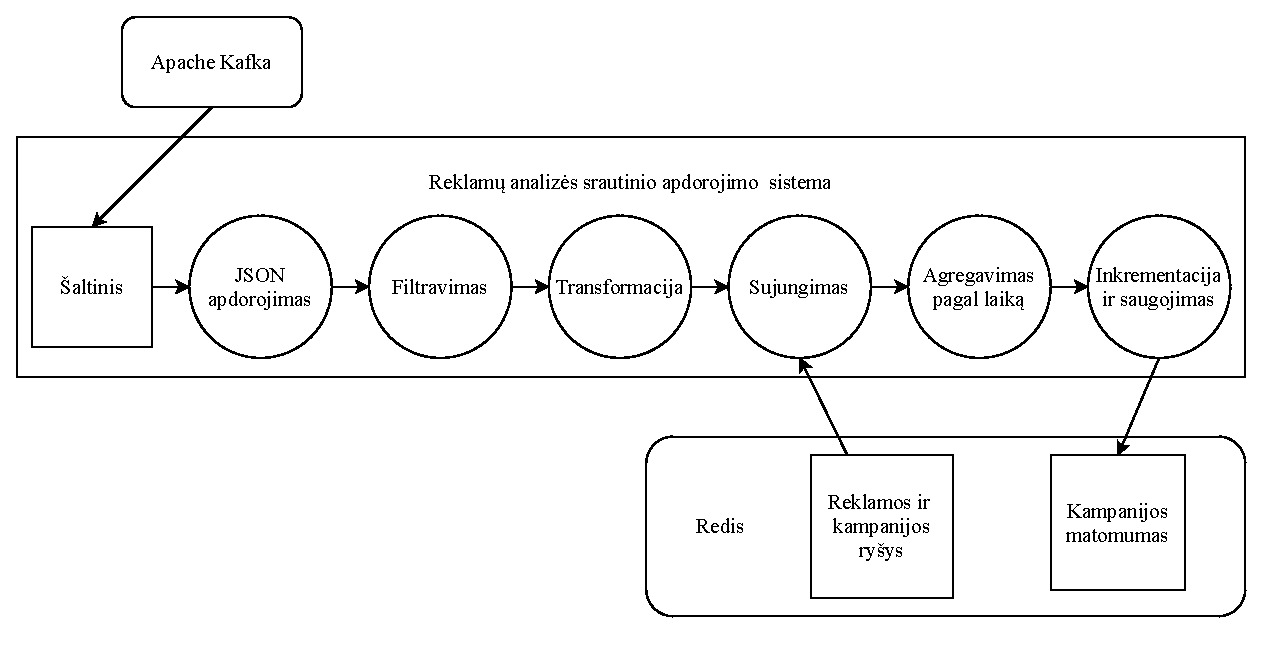
\includegraphics[width=15cm]{img/yahoo.pdf}
    \caption{Reklamų analizės sistema \cite{Chintapalli2016Benchmarking}}
    \label{yahoo}
\end{figure} 

\begin{figure}[H]
    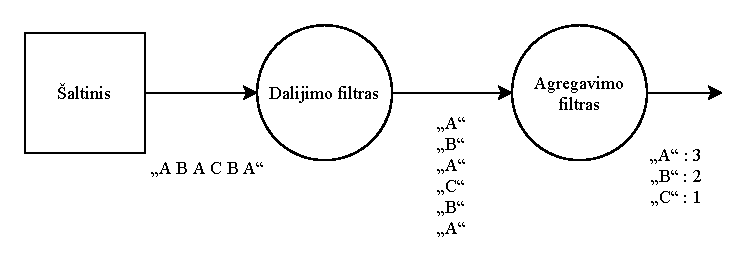
\includegraphics[width=15cm]{img/wordcount.pdf}
    \caption{WordCount sistemos pavyzdys}
    \label{wordcount}
\end{figure} 

Taip pat pagal MTDII literatūros analizę tyrimai bus atliekami su Reklamų analizės sistema (\ref{yahoo} pav.), kadangi ši sistema sukurta srautinių apdorojimo variklių vertinimui ir su WordCount srautinio apdorojimo sistemą (\ref{wordcount} pav.), kuri neturi pašalinių elementų sistemoje, kadangi Reklamų analizės sistema naudoja „Apache Kafka“, „Redis“ vertinimui.
Kadangi šios abi sistemos turi savo duomenų generavimo komponentus todėl jos bus naudojamos kaip tyrimo duomenis. Reklamų analizės sistema taip pat turi ir posisteme, kuri apskaičiuoją vėlinimą ir saugo jį tekstiniame įrašę, o WordCount sistemai įvertinti bus naudojama pačios Heron platformos įrašai siekiant kuo mažiau daryti įtakos rezultatams.

\subsection{Standartinė konfiguracija}
Sukurto sprendimo rezultatai bus lyginami su standartine konfiguracija tik su pakeistu skaičiavimo komponentų lygiagretumu atsižvelgiant į įrangos skaičiavimo gijų kiekį. Šiuo rezultatu bus tikrinama, ar Apache Heron pats negali taip pat arba geriau susitvarkyti su įeinančiu duomenų kiekiu nedidinant vėlinimo. Standartinės konfiguracijos naudojami balansavimo sprendimai \cite{twitterHeron}:
\begin{itemize}
    \item Srautinės apdorojimo sistemos priešslėgis (angl. backpressure) – kai pastebimas jog tam tikras skaičiavimo kompoenentas nespėja susidoroti su ateinančiu duomenu kiekiu ir praneša prieš tai einantiems skaičiavimo komponentams lėtinti duomenų patekimo greiiti. Heron yra implementuotas šaltinio priešslėgis, kuris veikia kaip buferis ant kiekvienos jungties tarp komonentų ir kai buferis prisipildo iki tam tikro taško įjungiamas priešslėgio režimas, kuris sulėtina srautinio apdorojimo sistemos greiti iki lėčiausio skaičiavimo komponento greičio. 
    \item Šiukšių surinktuvo (angl. garbage collector) optimizacija - kai srautinio apdorojimo sistema gaudavo dideli kiekį duomenų vienu metu ir užsipildydavo visa turima sistemos atmintis, kiekvieną karta gaunant nauja įraša buvo paleidžiamas šiukšlių surinktuvas, kuris naudoja daug resursų. Kad išspręsti šią problemą Heron periodiškai tikrina srautinio apdorojimo sistemos atminties talpą ir patenkančių duomenų dydį ir jeigu duomenų dydis pasidaro didesnis nei talpa tai duomenų paėmimo greitis sumažinamas per pusę ir taip kartojama kol pasiekiamas stabilus greitis. 
    \item Resursų rezervacija - kiekvienas konteineris (komponentų rinkinys) turi jam priskrita resursų kiekį ir prieš palaiedžiant srautinio apdorojimo sistema Heron rezervuoja reikiamus resursus ir jeigu komponentai bando pasiekti daugiau resursu negu jiems rezervuota yra lėtinama sistema taip užtikrinant stabilumą \cite{fu2015streaming}.  
\end{itemize}
\subsection{Balansavimas naudojant REINFORCE algoritmą}
Sukurtas sprendimas naudojantis Deep Q network ir Actor-Critic taip pat bus lyginamas su \cite{vaquero2018autotuning} aprašytų REINFORCE algortimu. Staripsnis nagrinėja automatinį balansavimą srautinio apdorojimo sistemų Apache Spark platformoje. Straipsnyje nagrinėjamas sprendimas susidaro iš trijų sistemų:
\begin{enumerate}
    \item Sistema, kurioje uš anksto sugeneruoti konfiguracijų deriniai leidžiami srautinio apdorojimo sistemose ir surenkamos metrikos bei konfiguracijos įverčiai. Gauti duomenis analyzuojami naudojant Factor Analysis + k-means ir gaunamas sąrašas pagrindinių metrikų bei konfiguracijos elementai darantys daugiausiai įtakos greitaveikai. Ši sistema naudojama vieną kartą prieš leidžiant sekančią sistemą. 
    \item Sistema, kurioje surinktos metrikos ir konfiguracijos elementai yra leidžiami iš naujo ir naudojant Lasso path analizę konfiguracijos elementų sąrašas surušiuojamas pagal įtaką greitaveikai. Tai daroma siekiant statistiškai užtikrinti, jog pasirinkti konfiguracijos elementai yra įtakingiausi. Ši sistema naudojama vieną kartą prieš leidžiant sekančią sistemą.
    \item Pagrindinė mašininio mokymosi sistema, naudojanti REINFORCE algoritmą, kuri naudodamas surikiuotų konfiguracijos elementų sąrašą ir pagrindinių metrikų sąraša periodiškai atnaujina konfiguraciją. Ši sistema paleidžiama tuo pačiu metu kaip ir srautinio apdorojimo sistema ir veikia visą laiką, kol paleistas ekspermientas.
\end{enumerate}  
Eksperimentinis sprendimas buvo sukonfiguruotas kas 5 minutes atnaujinti vieną konfiguracijos elementą. Autoriams pavyko pasiekti 70\% sumažinta vėlinimmą po 50 minučių ir mokymas pilnai konvergavo po 11 valandų. Magistro darbe bus naudojamas supaprastintas eksperimentas: bus implementuojamas REINFORCE algoritmas ir lyginamas su Deep Q Network ir Actor Critic algoritmais.

\sectionnonum{Išvados}

\printbibliography[heading=bibintoc] 

\end{document}
